\chapter{Specifikace požadavků}

Zadání této práce vzniklo původně z požadavku na rozšíření již fungující mobilní aplikace Catcher.
Její autor mne na konci roku 2015 oslovil s nápadem vylepšit její serverou část a doplnit API,
které by mohla využívat libovolná klientská aplikace. Po rychlé analýze jsme však oba došli k závěru,
že bude lepší navrhnout nový backend, protože ten starý nebyl reálně vůbec rozšiřitelný. %Jméno projektu je pojmenované po...

Finálním řešením je tak webová služba, která poskytuje kompletní rozhraní,
tzn. že jde o zcela nezávislou vrstvu mezi frontendem a backendem.
Protože výsledek mé práce má později nahradit nevyhovující backend staré aplikace, ponechal jsem celému projektu jméno Catcher.

\section{Požadavky na Catchera}

Protože se v komunitě hráčů i organizátorů turnajů jako aktivní hráč sám pohybuji,
nebyl problém stanovit funkční i nefunkční požadavky na vznikající službu.

\subsection{Funkční požadavky}

\begin{description}
  \item[Import a export dat]
    Systém umožňuje import oddílů a jeho hráčů z databáze ČALD.
  \item[Rozpis zápasů]
    Oprávněná role může vytvořit svůj vlastní turnaj a vložit seznam všech zápasů,
    které se budou hrát. Vytvořený rozpis zápasů systém již doplňuje automaticky na základě
    odehraných výsledků (např.~vítěze semifinále automaticky posune do finále). Ve chvíli,
    kdy to bude již možné, doplní celkové pořadí turnaje. Automatické doplnění se týká i 
    souhrnné tabulky vzájemných hodnocení v kategorii SOTG.
  \item[Zadávání dat v rámci turnaje]
    Každý tým má možnost vytvořit vlastní soupisku na turnaj. Systém pak umožňuje
    v průběhu turnaje zadávat konkrétní údaje:
    \begin{itemize}
      \item průběžné skóre zápasů nebo jejich závěrečný výsledek
      \item skórující a asistující hráč
      \item hodnocení SOTG
    \end{itemize}
  \item[Tvorba statistik]
    Systém tvoří detailní statistiky hráčů, týmů a zápasů (obdržené a udělené body,
    počet asistencí, průměrná hodnota SOTG).
\end{description}

\subsection{Nefunkční požadavky}

\begin{description}
  \item[Snadná rozšířitelnost]
    Už nyní evidujeme změny, o které je zájem, ale nejsou předmětem této práce.
    I proto je nutné projekt dokončit tak, aby byl v budoucnu snadno rozšiřitelný nebo
    modifikovatelný.
  \item[Nízká cena]
    Cílem není vytvořit výdělečný projekt, ale fungující službu pro několik stovek hráčů
    a fanoušku v České republice. I proto je požadavkem použití volně dostupných
    knihoven a technologií.
  \item[Výkon]
    Podle celkem jednoduchých odhadů lze usoudit, že aplikaci budou čekat výkyvy v provozu.
    Většina zápisů a čtění dat probíhá během samotných turnajů. Během špičky nebude počet požadavků za sekundu
    větší než několik desítek. I proto není na celkový výkon kladen žádný zvláštní požadavek.
    Systém by každopádně měl minimálně 95 \% žádostí zpracovat do jedné sekundy.
  \item[Spolehlivost]
    Spolehlivost je základem pro funkční běh Catchera. Velká část operací, včetně chybných budou
    zapisovány do souborů pro snadné odhalení chyb. Obnova musí být proveditelná ze zálohovacích souborů.
    %V případě výpadku by měl být informován administrátor pomocí SMS nebo e-mailu.
    \item[Bezpečnost]
    Systém musí jednoznačně určit a ověřit uživatele, který přistupuje k rozhraní Catchera. Zároveň
    musí existovat možnost za chodu přidávat, odebírat nebo měnit oprávnění uživatelů.
    % Dále pak systém musí být datově integritní, tzn. že obsah zpráv nebude při přenosu změněn.
    Pro tento projekt není nutné používat HTTPS\footnote{Hypertext Transfer Protocol Secure} protokol.
  \item[Nároky na hardware]
    Systém musí být schopen běžet na běžných serverech s ne více jak 1024 MB RAM\footnote{Random Access Memory}.
  \item[Formát importu]
    Pro import soupisek musí systém umět číst data ve formátu, který ČALD pro export používá.
  \item[Vytvoření dokumentace]
    Pro vývoj klientských aplikací je potřeba vytvořit dostatečně detailní dokumentaci rozhraní.
\end{description}

\section{Uživatelské role}

\begin{description}
  \item[Nepřihlášený návštěvník]
    Jde o nejčastější přístup k aplikaci. Slouží k zobrazení všech statistik (aktuální skóre,
    statistika všech hráčů, hodnocení SOTG). Nemůže žádná data vytvářet nebo modifikovat
    a nevyžaduje přihlášení.
  \item[Organizátor]
    Účet pod touto rolí může vytvořit kdokoliv pouhou registrací. Po příhlášení lze přídávat
    nové turnaje a ty následně spravovat. Tím se rozumí tvorba rozpisu zápasů a seznamu účastníků.
    Dále může zadávat průběžné a výsledné skóre zápasů, skórující a asistující hráče a vidí
    na tabulku vzájemných hodnocení SOTG pro účely vyhlášení vítěze.
    Tato tabulka je pro ostatní role až do ukončení turnaje nezobrazitelná.
  \item[Klubový/oddílový účet]
    Pro účely odevzdávání hodnocení SOTG a úprav v týmové soupisce je vytvořen pro každý oddíl
    jeden společný účet. Tento účet má možnost vytvořit pouze administrátor. Přihlašovací údaje pak
    získá zástupce klubu a je pouze na něm, kdo z jeho oddílu bude spravovat vytvořený učet.
    Součástí klubu může být více týmů, např. mužský a~ženský tým nebo A-tým a B-tým.
  \item[Administrátor]
    Má plnou kontrolu nad správou účtů a nad daty v databázi.
    Jeho možnosti vznikají sjednocením všech ostatních rolí.
\end{description}

\section{Případy užití}
\label{sec:use_case}

Následující část popisuje nejběžnější případy užití. V návrhu rozhraní jde
o~jednu z~nejdůležitejších součastí, protože určuje směr návrhu. Výsledné API by tak mělo
pokrývat všechny níže uvedené případy. Seznam zachycuje jednotlivé požadavky
a~jejich popis:

\subsection*{Import}
  \begin{description}
    \item[UC1: Import dat z databáze ČALD]
      Doplňuje seznam oddílů a jejich hráčů do databáze Catchera. Manuálně lze stáhnout
      aktuální data z ČALD databáze a doplnit doposud aktuální data v databázi.
  \end{description}

\subsection*{Uživatelé}
  \begin{description}
    \item[UC2: Registruje nového uživatele]
      Kdokoliv se může stát registrovaným uživatelem s rolí organizátor. Stačí se zaregistrovat s platným e-mailem.
      Klubové účty vytváří administrátor.
    \item[UC3: Autentizuje uživatele]
      Určí skutečnou identitu uživatele. Jinými slovy jej přihlásí. Po úspěšném přihlášení je uživateli vrácen
      přístupový token pro vykonávaní dalších požadavků (více k sekci~\ref{sec:security}).
    \item[UC4: Odesílá zapomenuté heslo]
      Při ztrátě hesla lze požádat o odeslání nového náhodně vygenerovaného na e-mail, který uživatel zadal při své registraci.
  \end{description}

\subsection*{Oddíly}
  \begin{description}
    \item[UC5: Vytvoří oddíl]
      Uloží nový oddíl do databáze. Ukládá se u~něj jméno, město a~země původu.
    \item[UC6: Získá oddíly]
      Vrátí informace o jednom nebo více oddílech.
    \item[UC7: Edituje oddíl]
      Upraví informace o oddílu.
    \item[UC8: Smaže oddíl]
      Smaže oddíl z databáze.
  \end{description}

\subsection*{Hráči}
  \begin{description}
    \item[UC9: Vytvoří hráče]
      Vytvoří nového hráče, u kterého lze vytvořit vazba pouze k jednomu oddílu.
      Kromě jména a příjmení u něj lze uložit číslo dresu a jeho přezdívku.
    \item[UC10: Získá hráče]
      Vrátí informace o jednom nebo více hráčích.
    \item[UC11: Edituje hráče]
      Upraví informace o hráči.
    \item[UC12: Smaže hráče]
      Smaže hráče z databáze.
  \end{description}

\subsection*{Týmy}
  \begin{description}
    \item[UC13: Vytvoří tým]
      Vytvoří tým spadající pod konkrétní oddíl. Týmu se musí přiřadit stupeň a divize (např. A-tým ženy).
    \item[UC14: Získá týmy]
      Vrátí informace o jednom nebo více týmech.
    \item[UC15: Edituje tým]
      Upraví informace o týmu.
    \item[UC16: Smaže tým]
      Smaže tým z databáze.
  \end{description}

\subsection*{Turnaje}
  \begin{description}
    \item[UC17: Vytvoří turnaj]
      Uloží nový turnaj včetně účastníků turnaje, základních skupin a zápasů ve skupinách a play-off.
    \item[UC18: Edituje turnaj]
      Upraví informace o turnaji nebo změní jeho stav.
    \item[UC19: Získá turnaje]
      Vrátí informace o jednom nebo více turnajích.
    \item[UC20: Získá konečné pořadí]
      Získá známé pořadí týmů na turnaji a pokud turnaj již skončil, zobrazí i hodnocení SOTG.
  \end{description}

\subsubsection*{Týmové soupisky}
  \begin{description}
    \item[UC21: Připsat hráče na soupisku]
      Týmům na turnaji lze přiřadit hráče, tzn. vytvořit týmové soupisky. Hráčům ze soupisky
      pak lze připisovat body na turnaji. Každý hráč může hrát na turnaji pouze za jeden tým.
    \item[UC22: Získá soupisky]
      Vrátí soupisku konkrétního týmu nebo seznam hráčů napříč celým turnajem. Včetně jejich statistik a seřazení dle úspěšnosti.
    \item[UC23: Odebere hráče ze soupisky]
      Jestliže hráč nedisponuje žádnými statistikami a nestihl ještě do žádného zápasu zasáhnout, je možné jej odstranit ze soupisky.
  \end{description}

\subsubsection*{Skupiny a zápasy}
  \begin{description}
    \item[UC24: Získá skupiny]
      Vrátí informace o vybraných skupinách. Seznam týmů včetně jejich vzájemného skóre a pořadí ve skupině.
    \item[UC25: Získá zápasy]
      Vrátí stav, výsledné skóre, nebo hodnocení SOTG vybraných zápasů.
    \item[UC26: Upraví zápas]
      Umožňuje zahájit nebo ukončit zápas. Dále lze editovat výsledné skóre nebo hřiště, na kterém se bude hrát.
    \item[UC27: Vytvoří nový bod v zápase]
      Každý bod, který se odehraje, může evidovat skórujícího a nahrávajícího hráče a informaci, zda šlo o bod typu Callahan\footnote{
      Body, při kterých skórujícímu hráči nahraje soupěř, jsou označovány jako Callahan.
      Když využijeme hokejovou terminologii, je to něco jako vlastní gól.}.
    \item[UC28: Smaže body v zápase]
      V případě potřeby lze smazat dříve vložené body.
  \end{description}

\subsubsection*{SOTG na turnaji}
  \begin{description}
    \item[UC29: Ohodnotí soupeře v daném zápase hodnocením SOTG]
      Po~každém zápase může uživatel z klubového účtu ohodnotit soupeře hodnocením SOTG.
      Toto hodnocení se skládá z několika bodovaných kategorií.
      V celkovém součtu jde o hodnocení na stupnici od 0 do 20.
    \item[UC30: Upraví již jednou odevzdané hodnocení SOTG]
      Před~ukončením turnaje umožňuje změnit hodnocení.
    \item[UC31: Získá všechna odevzdaná hodnocení SOTG]
      Do~ukončení turnaje viditelné pouze pro organizátora.
    \item[UC32: Získá všechna neodevzdaná hodnocení SOTG]
      Před ukončením turnaje lze zkontrolovat, zda jsou všechna hodnocení již odevzdaná.
      V~opačném případě zobrazí seznam týmů, které hodnocení neodevzdaly.
  \end{description}

\begin{figure}[ht!]
\centering
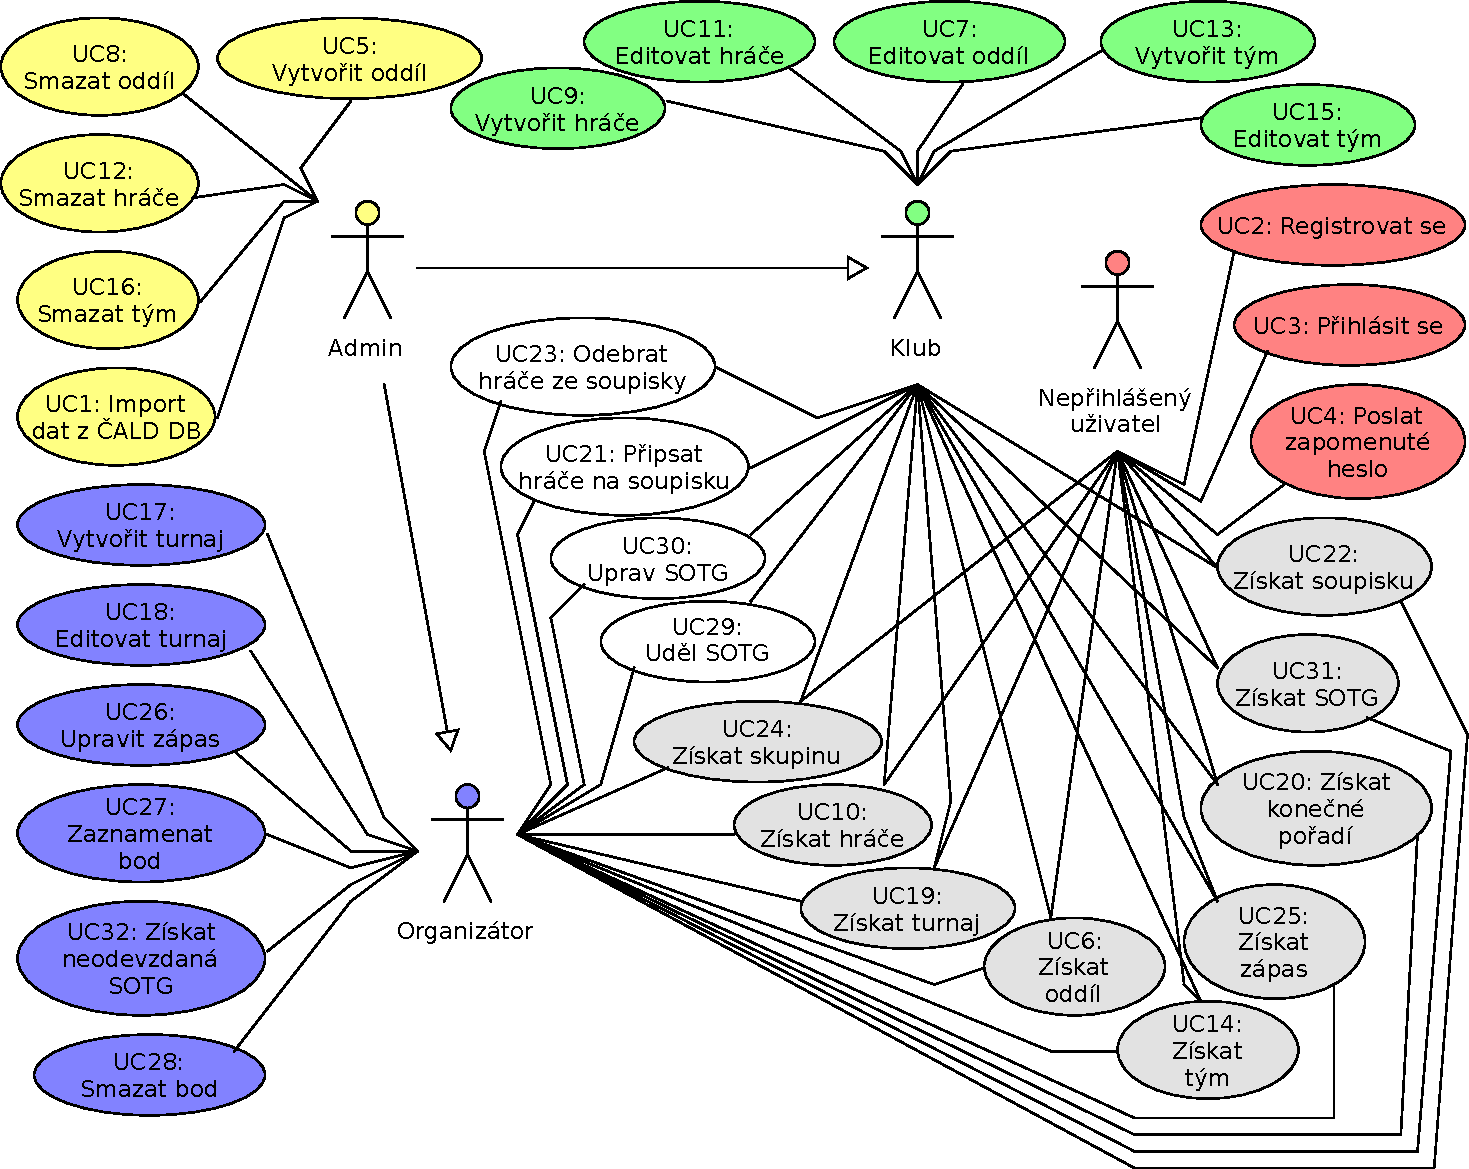
\includegraphics[width=130mm]{./images/use-case.pdf}
\caption{Use case diagram\label{overflow}}
\end{figure}
